\documentclass{beamer}

\usetheme{metropolis}

%\usepackage%[format=plain,indention=1cm,scriptsize,font=sf ,labelfont=bf,
%  nooneline]{caption}
\usepackage{subcaption}
%\usepackage{subfig}
\usepackage[ngerman]{babel}
\usepackage[utf8x]{inputenc}
\usepackage{verbatim}
\usepackage{epstopdf}
%\usepackage[floatrow]{chemstyle}

\begin{document}

\title{\vspace*{2.0cm}Top-tagging durch track-basierte Substrukturanalyse}
\author[Nicolas Lang]{Nicolas Lang} %, Peter Mättig}
\institute{
Bergische Universit\"at Wuppertal\\
\includegraphics[width=0.2\textwidth,valign=t]{img/bmbf.png}
}
\date{\today}

\titlegraphic{\includegraphics[width=1.0\textwidth]{img/FSP103.png}%\hspace*{4.75cm}~%
   %\includegraphics[width=2cm]{logopolito}
}

\maketitle


%\setbeamertemplate{footnote}{%
%\parindent 0em\noindent%
%\raggedright
%\usebeamercolor{footnote}\hbox to 0.8em{\hfil\insertfootnotemark}\insertfootnotetext\par%
%}

\setbeamertemplate{frame footer}{\tiny{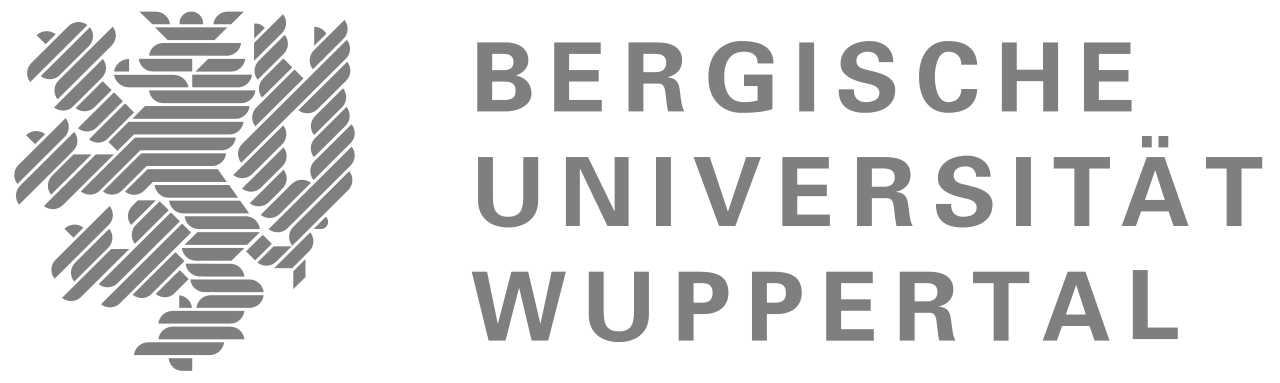
\includegraphics[width=0.1\textwidth]{img/BUW_Logo.png} \qquad Nicolas Lang, Bergische Universit\"at Wuppertal}}


% ==##==##==##==##==##==##==##==##==##==##==##==##==##==##==##==##==##==##==##==##

\begin{comment}
\begin{frame}
    \frametitle{Content}
    %\begin{itemize}
    %   \item Bla
    %\end{itemize}
    %\content
\end{frame}
\end{comment}



%\section*{Die Bedeutung geboosteter top quarks}

\begin{frame}
    \frametitle{Standardmodell - vollständige Beschreibung der Natur?}
    \begin{itemize}
        \item 2012: Higgs entdeckt - Teilchenzoo des Standardmodells vollständig, aber ...
        \item das Standardmodell lässt einige Fragen unbeantwortet (Neutrinomassen, Higgsmassen fine-tuning, Gravitation?...)
        \item $\Rightarrow$ unvollständige Beschreibung der Natur
        \item $\Rightarrow$ Physik jenseits des Standardmodells (BSM)
    \end{itemize}
\end{frame}

\begin{frame}
    \frametitle{Suche nach neuer Physik}
    \begin{itemize}
        \item Vorhersage (z.B. SuSy): neue (schwere) Teilchen zerfallen in schwerstes Standardmodell Teilchen: das Top Quark
        \item schwere Teilchenzerfälle bedingen hohe Transversalimpulse (Boosts)
        \item $\Rightarrow$ geboostete Top Quarks wichtiges Signal in vielen BSM Analysen
        \item LHC energetisch in guter Ausgangsposition für BSM Messungen
    \end{itemize}
\end{frame}

\begin{frame}
    \frametitle{Top Tagging in geboosteten Umgebungen}
    \begin{itemize}
        \item hadronischer Top Zerfall: $t \rightarrow W + b \Rightarrow u + d + b$
        \item resolved: 3 Jets im Final State
        \item boosted: 1 Fatjet (large-radius Jet)
        \item größter Untergrund: harte Initial- / Final State Radiation (ISR/FSR)
        \item wie unterscheiden? Substruktur des Fatjets!
    \end{itemize}
\end{frame}



%%%TODO: hier muss noch ein Feynman Diagramm vom Top Zerfall her
%\section*{Track-basierte Substrukturanalyse}

\begin{frame}
    \frametitle{Motivation: Gluon Splitting Funktion}
    \begin{itemize}
        \item die Wahrscheinlichkeit von Gluonstrahlung mit Impulsanteil $(1-z)$ ist
        \begin{equation}
            P_{gq} = \frac 4 3 \left( \frac {1 + z^2} {1 - z} \right)
        \end{equation}
        $\Rightarrow$ Gluonstrahlung ist meist kollinear und weich
        \item harte Zerfälle ($W$, top): flache z Verteilung, $\langle z \rangle = 0.5$
        \item Observablen sensitiv auf $p_T$ und Winkel gute Diskriminanten
    \end{itemize}
\end{frame}

\begin{frame}
    \frametitle{Kurzer Exkurs: Jet Algorithmen}
    \begin{itemize}
        \item Jet Algorithmen können auf Kalorimeter Cluster, Tracks und Truth Teilchen angewendet werden
        \item Sequential-Recombination Algorithmen (inclusive):
        \begin{itemize}
            \item finde kürzeste Distanz zwischen zwei Protojets bzw. Protojet und Beam bzgl. definierter Metrik
            \item kombiniere die Protojets oder erkläre Protojet zu fertigem Jet, falls Beamdistanz am kürzesten
            \item wiederhole dies, bis nur noch Jets vorhanden sind
        \end{itemize}
        \item $k_T$-Algorithmus benutzt die Metrik
        \begin{equation}
            d_{ij} = \text{min}(p_{Ti}^2,p_{Tj}^2) \left(\frac{\Delta R_{ij}}{R}\right)^2
        \end{equation}
        $\rightarrow$ kehrt Partonsplitting um
    \end{itemize}
\end{frame}

\begin{frame}
    \frametitle{Anwendung auf ghost-assoziierte Tracks}
    \begin{itemize}
        \item Ghost-Association: Tracks werden (Fat-)jets zugeordnet, indem sie im Clusterprozess mitberücksichtigt werden, aber mit winzigem Transversalimpuls ($\sim 10$ eV)
        \item $\rightarrow$ robuster als $\Delta R$ matching
        \item $k_T$-Algorithmus wird auf ghost-assoziierte Tracks angewendet, mit kleinem Jetradius ($R = 0.2$). Vorteil: Pile-up/underlying event kann durch Matching zum Primary Vertex stark reduziert werden
    \end{itemize}
\end{frame}

\begin{frame}
    \frametitle{Substrukturanalyse}
    \begin{itemize}
        \item Substrukturanalyse basiert auf den so erhaltenen ''Ghost-jets''
        \item Subjets werden zu Paaren gruppiert - $(N_{\text{subj.}})!$ Möglichkeiten. Ziel: Identifikation des $W$-Paares ($u+d$, $s+c$)-Jets
        \item wir betrachten 3 Gruppen von Variablen: massen-bezogene Variablen, colourflow-sensitive Variablen, und Jetladung
        \item die Subjets werden zur Kontrolle mit den generator-level Partonen assoziiert
        \item alle Distributionen werden für $W$-Paare, Paare mit $b$-Jets und untergrund-artige Paare von Subjets betrachtet
    \end{itemize}
\end{frame}

%%%damit:

\begin{frame}
    \frametitle{$k_T$ Maß und Jetmasse}
    \begin{itemize}
        \item track-basierte Jetmasse:
        \begin{equation}
            m_{\text{Jet}}^2 = \big(\sum_{i \in \text{subjet}}{p_i}\big)^2 \times E_{\text{fatjet}} / E_{\text{tracks}}
        \end{equation}
        \item $k_T$-Maß des letzten Rekobinationsschrittes lässt ebenfalls Rückschlüsse auf Masse des Zerfalls zu:
        \begin{equation}
            \sqrt{d_{ij}} \approx \sqrt{ \frac {x}{1-x} } m
        \end{equation}
        \item $\Rightarrow$ beide Variablen sind stark korreliert
    \end{itemize}
\end{frame}

\begin{frame}
    \frametitle{$k_T$ Maß und Jetmasse}
    \begin{minipage}[c]{0.48\linewidth}
    \begin{figure}
        \begin{subfigure}[t]{1.0\linewidth}
            %\centering
            \includegraphics[width=1.0\textwidth]{img/ghostjetPairs/gt125/mass/fatjetIsT.eps}
        \end{subfigure}
        \begin{subfigure}[t]{1.0\linewidth}
            %\centering
            \includegraphics[width=1.0\textwidth]{img/ghostjetPairs/gt125/kt/fatjetIsT.eps}
        \end{subfigure}
    \end{figure}
    \end{minipage}
    \hfill
    \begin{minipage}[c]{0.48\linewidth}
        \begin{itemize}
            \item $k_T$-Distanz: breiter Peak um $m_W/2$ für $W$-Paare
            \item Jetmasse: deutlicher Peak bei $W$-Masse, klein für Untergrund
        \end{itemize}
    \end{minipage}
\end{frame}


\begin{frame}
    \frametitle{Komplementärer Ansatz: Jet Ladung}
    \begin{itemize}
        \item hadronischer Topjet hat charakteristische Ladungskonfiguration
        \item semi-leptonische Zerfälle: hadronische $W$-Ladung entgegengesetzt zu Lepton-Ladung $\Rightarrow$ multipliziere Jetladung mit Lepton Ladung
        \item Jetladung (basiert auf Ladung der Hadronen und Fragmentationsfunktionen)
    \end{itemize}
    \begin{equation}
        Q_{Jet} = \sum_{i \in  \text{jet} } q_{i} \left(\frac{p_{T, i}}{p_{T, \text{jet}}}\right)^{\alpha} 
    \end{equation}
\end{frame}

\begin{frame}
    \frametitle{Jet Ladung}
    \begin{minipage}[c]{0.50\linewidth}
    \begin{figure}
        %\begin{subfigure}
            %\centering
            \includegraphics[width=1.0\textwidth]{img/ghostjetPairs/gt125/charge/charge.eps}
        %\end{subfigure}
        %\begin{subfigure}
            %\centering
            %\includegraphics[width=0.6\textwidth]{img/ghostjetPairs/gt125/kt/fatjetIsT.eps}
        %\end{subfigure}
    \end{figure}
    \end{minipage}
    \hfill
    \begin{minipage}[c]{0.48\linewidth}
        \begin{itemize}
            \item deutlicher Offset für $W$-Paare
            \item leichter Offset beim Untergrund durch $b$-Jet der leptonischen Seite
        \end{itemize}
    \end{minipage}
\end{frame}



\begin{frame}
    \frametitle{Weiteres Merkmal: Colourflow und Multiplizität}
    \begin{itemize}
        \item $W$-Zerfall: Farbsingulett - Farbindizes kontrahiert
        \item Strahlungshäufung zwischen $u$- und $d$-Jets erwartet
        \item betrachte:
        \begin{itemize}
            \item Multiplizität (ggf. $p_T$-gewichtet)
            \item Dipolarity: wie weit ist Strahlung von der Achse zwischen zwei Subjets entfernt
            \begin{equation}
                \mathcal{D} = \frac 1 {R_{12}^2} \sum_{i \in \text{ fatjet}} \frac {p_{T,i}} {p_{T,{\text{fatjet}}}} R_i^2
            \end{equation}
            ($R_i$ = Abstand zur Achse, $R_{12}$ = Abstand der Subjets)
        \end{itemize}
    \end{itemize}
\end{frame}

\begin{frame}
    \frametitle{Colourflow und Track-Multiplizität}
    \begin{minipage}[c]{0.48\linewidth}
    \begin{figure}
        \begin{subfigure}[b]{1.0\linewidth}
            %\centering
            \includegraphics[width=1.0\textwidth]{img/ghostjetPairs/gt125/mult/fatjetIsT0.eps}
        \end{subfigure}
        \begin{subfigure}[b]{1.0\linewidth}
            %\centering
            \includegraphics[width=1.0\textwidth]{img/ghostjetPairs/gt125/dip/other.eps}
        \end{subfigure}
    \end{figure}
    \end{minipage}
    \hfill
    \begin{minipage}[c]{0.48\linewidth}
        \begin{itemize}
            \item Dipolarity: langer Tail der Untergrundverteilung (Effekt klein)
            \item höhere Multiplizität bedingt durch höheres $p_T$
        \end{itemize}
    \end{minipage}
\end{frame}


\begin{frame}
    \frametitle{Die Suche nach dem W-Zerfall...}
    \begin{itemize}
        \item fasse Informationen zusammen in multivariater Diskriminante: Gewinne $W$-Likelihood aus Distributionen der Substrukturvariablen für jedes Paar:
        \begin{equation}
            y_{\mathcal{L}}(x) = \frac {\mathcal{L}_S(x)} {\mathcal{L}_S(x) + \mathcal{L}_B(x)}
        \end{equation}
        \item identifiziere Paar mit höchstem $y_{\mathcal{L}}$-Wert mit $W$-Zerfall
        \item $b$-Tagging zur Untergrundreduktion (viele Distributionen ähnlich für $W$ und $b$)
    \end{itemize}
\end{frame}


\begin{frame}
    \frametitle{Vorläufige Ergebnisse und Ausblick}
    \begin{itemize}
        \item Identifizierung des $W$-Zerfalls unter den Subjet-Paaren mit $80.2\%$ Effizienz
        \item verbesserte Massenauflösung durch kleinen Subjetradius
        \item Ausblick: Kombination der track-basierten Substrukturinformation mit Fatjetkinematik in BDT
    \end{itemize}
\end{frame}



\begin{comment}
\begin{frame}
    \frametitle{}
    \begin{minipage}[b]{0.48\linewidth}
    \begin{figure}
        %\centering
        %\includegraphics[width=0.6\textwidth]{img/shaun1.png}
    \end{figure}
    \end{minipage}
    \hfill
    \begin{minipage}[b]{0.48\linewidth}
        \begin{itemize}
            \item 
        \end{itemize}
    \end{minipage}
\end{frame}
\end{comment}


%\begin{comment}
%\begin{frame}
%    \frametitle{References} 
    %\bibliographystyle{amsalpha} 
    %\bibliography{bibliography}

    %\begin{comment}
    %\begin{thebibliography}{20}
%        \providecommand{\url}[1]{\texttt{#1}}
%        \providecommand{\urlprefix}{URL }
        
%        \setbeamertemplate{bibliography item}[online]
%        \bibitem{url:django}
%        \emph{The Web framework for perfectionists with deadlines | Django},
%        \textbf{2014}.
%        \newblock \urlprefix\url{https://www.djangoproject.com}.

%        \setbeamertemplate{bibliography item}[article]
%        \bibitem{rivet}
 %       Andy Buckley et~al.
 %       \emph{Rivet User Manual},
  %      arXiv:1003.0694 [hep-ph].

    %\end{thebibliography}
    %\end{comment}
    
%\end{frame}
%\end{comment}


% ==##==##==##==##==##==##==##==##==##==##==##==##==##==##==##==##==##==##==##==##


\end{document}
